\documentclass[12pt, UTF8, a4paper]{ctexart}
\usepackage{morelull}
\usepackage{graphicx}
\usepackage{booktabs}
\usepackage{threeparttable}

\title{研究生留学申请数据分析}
\author{2018011365 张鹤潇}
\date{\today}

\begin{document}

\begin{titlepage}
    
\maketitle

\begin{abstract}
    本科生在为研究生留学申请做准备时常常陷入迷茫:
    录取竞争力与什么因素有关?科研经历有多重要?
    本文通过分析相关数据回答了这些问题,并
    利用线性回归、决策树等机器学习方法建模,
    在保证可解释性的前提下,尽可能准确地预测申请成功的概率,
    以期为申请者提供决策依据。
\end{abstract}
\tableofcontents

\thispagestyle{empty}
\end{titlepage}

\setcounter{page}{1}

\section{研究背景}

研究生留学申请是一次重要的人生选择,
申请者为了提高自己的竞争力常要投入经年累月的努力。
遗憾的是,申请过程中的信息不对称往往造成资源和精力的浪费:
学长的经验难免失之偏颇,大学排名和中介机构又有误导性。
鉴于此,作为一名在读本科生,我很想解决如下几个问题:
\begin{itemize}
    \item 研究生留学录取概率与什么因素有关?
    \item 各个因素,尤其是科研经历的重要性有多大?
    \item 能否根据个人信息预测录取概率?
\end{itemize}

\section{数据分析}

\subsection{数据集介绍}

本项研究的原始数据包含了500位申请者的各项指标及其被录取的概率。

\begin{table}[htbp] 
    \caption{\label{tab:1}部分研究数据} 
    \centering
    \small
    \begin{tabular}{cccccccc} 
     \toprule 
     GRE & TOEFL & Univ. Rating & SOP & LOR & GPA & Research & Chance of Admit \\ 
     \midrule 
    327 & 117 & 4 & 4.5 & 4.5 & 3.86 & 1 & 0.92\\
    324 & 107 & 4 & 4.0 & 4.5 & 3.55 & 1 & 0.76\\
    316 & 104 & 3 & 3.0 & 3.5 & 3.20 & 1 & 0.72\\
     \bottomrule 
    \end{tabular}
\end{table}

对于各个特征的含义解释如下:

\begin{itemize}
    \item GRE: 美国研究生入学考试成绩,取值0-340;
    \item TOEFL: 托福考试成绩,取值0-120;
    \item Univ. Rating: 本科大学等级,最高为5;
    \item SOP:申请文书(Statement of Purpose),最高为5;
    \item LOR:推荐信力度(Letter of Recommendation Strength),最高为5;
    \item GPA:本科成绩平均绩点,原始数据为10分制,这里转为4分制;
    \item Research:是否有科研经历,取值0(无)或1(有);
    \item Chance of Admit: 研究生录取概率。
\end{itemize}

\subsection{描述性数据分析}

\begin{figure}[htb]
    \centering
    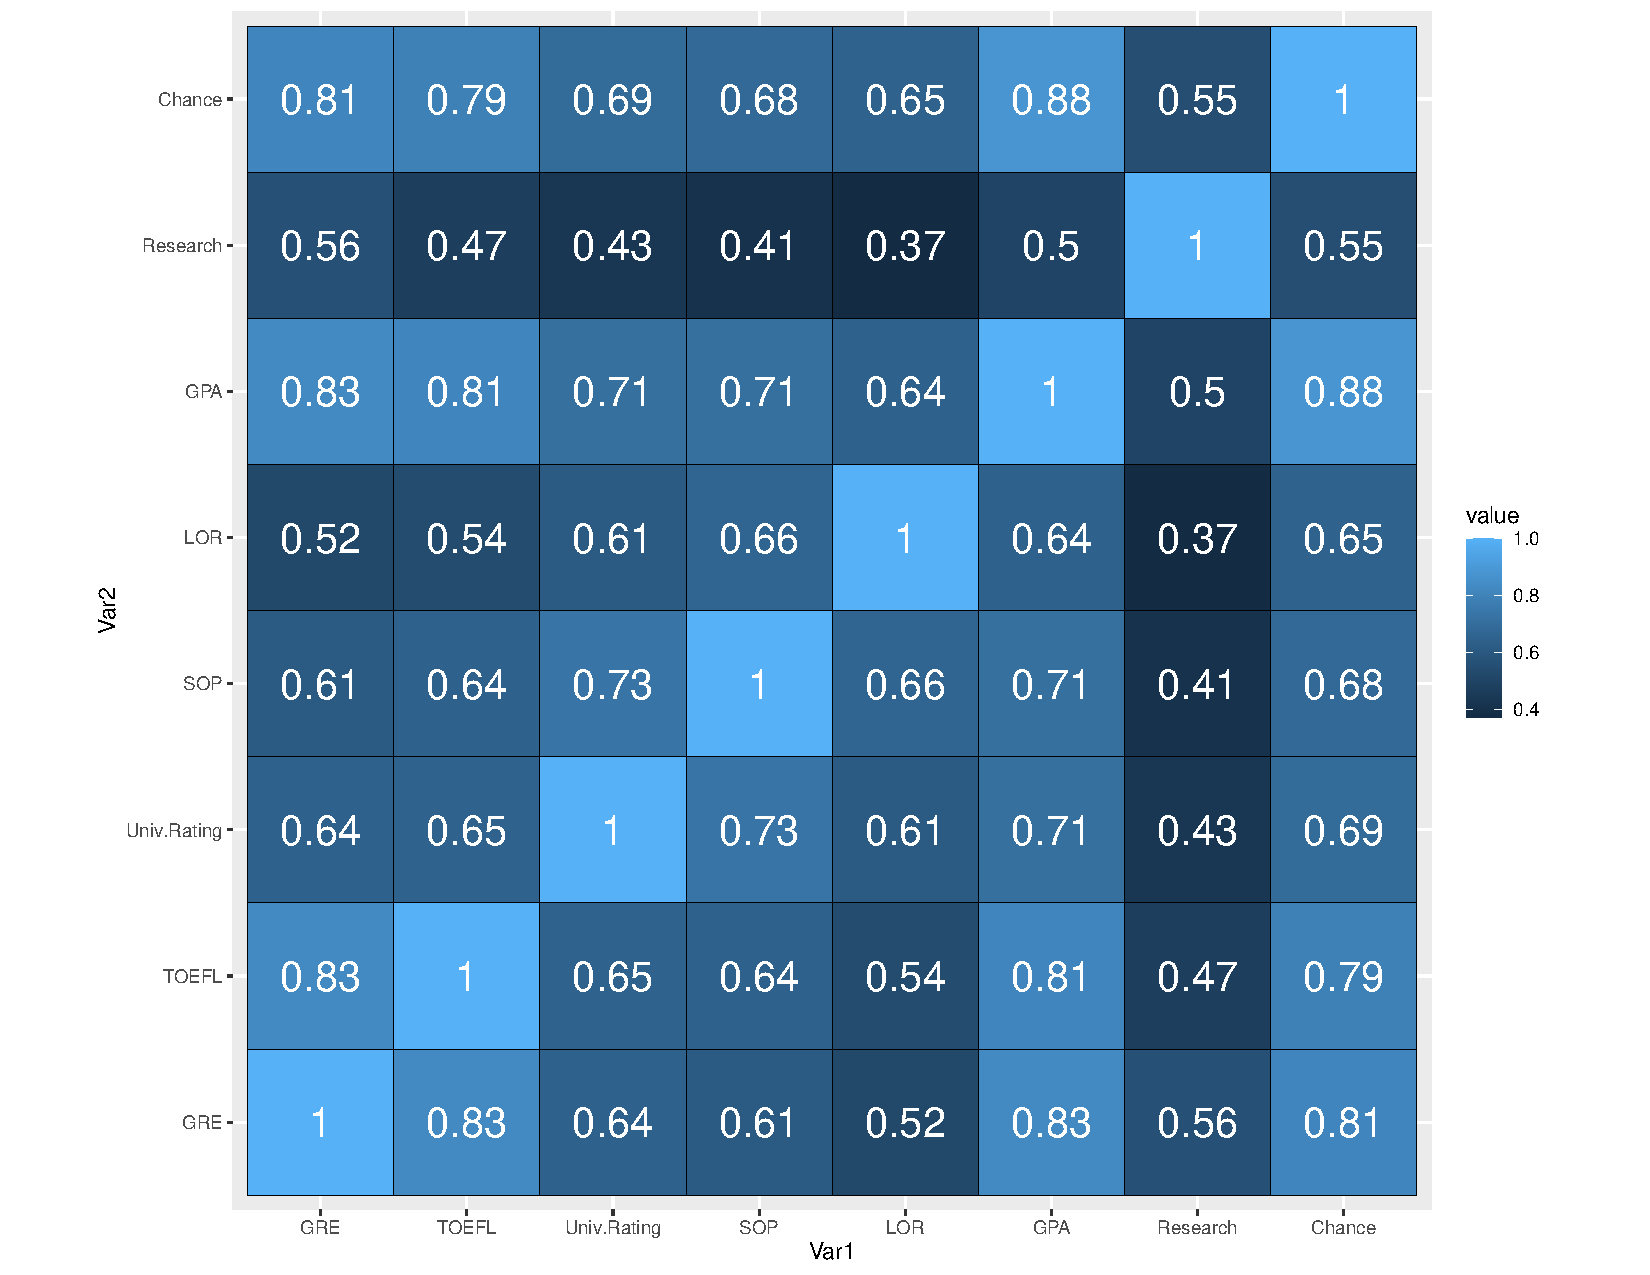
\includegraphics[width=4in, keepaspectratio]{./pic/corplot.pdf}\\
    \caption{相关系数矩阵图}
\end{figure}

由相关系数矩阵图可见,所有因素对于录取概率都有明显的贡献,尤以GPA为甚。
GPA、TOEFL、GRE成绩高度线性相关,也就是说,
本科成绩更好的申请者倾向于在英语考试中取得更高的分数,这是符合直觉的。
另外,所有特征之间都有显著的正相关关系,换句话说,在某个方面占据优势的申请者,
往往在其它方面也占优。

\begin{figure}[htb]
    \centering
    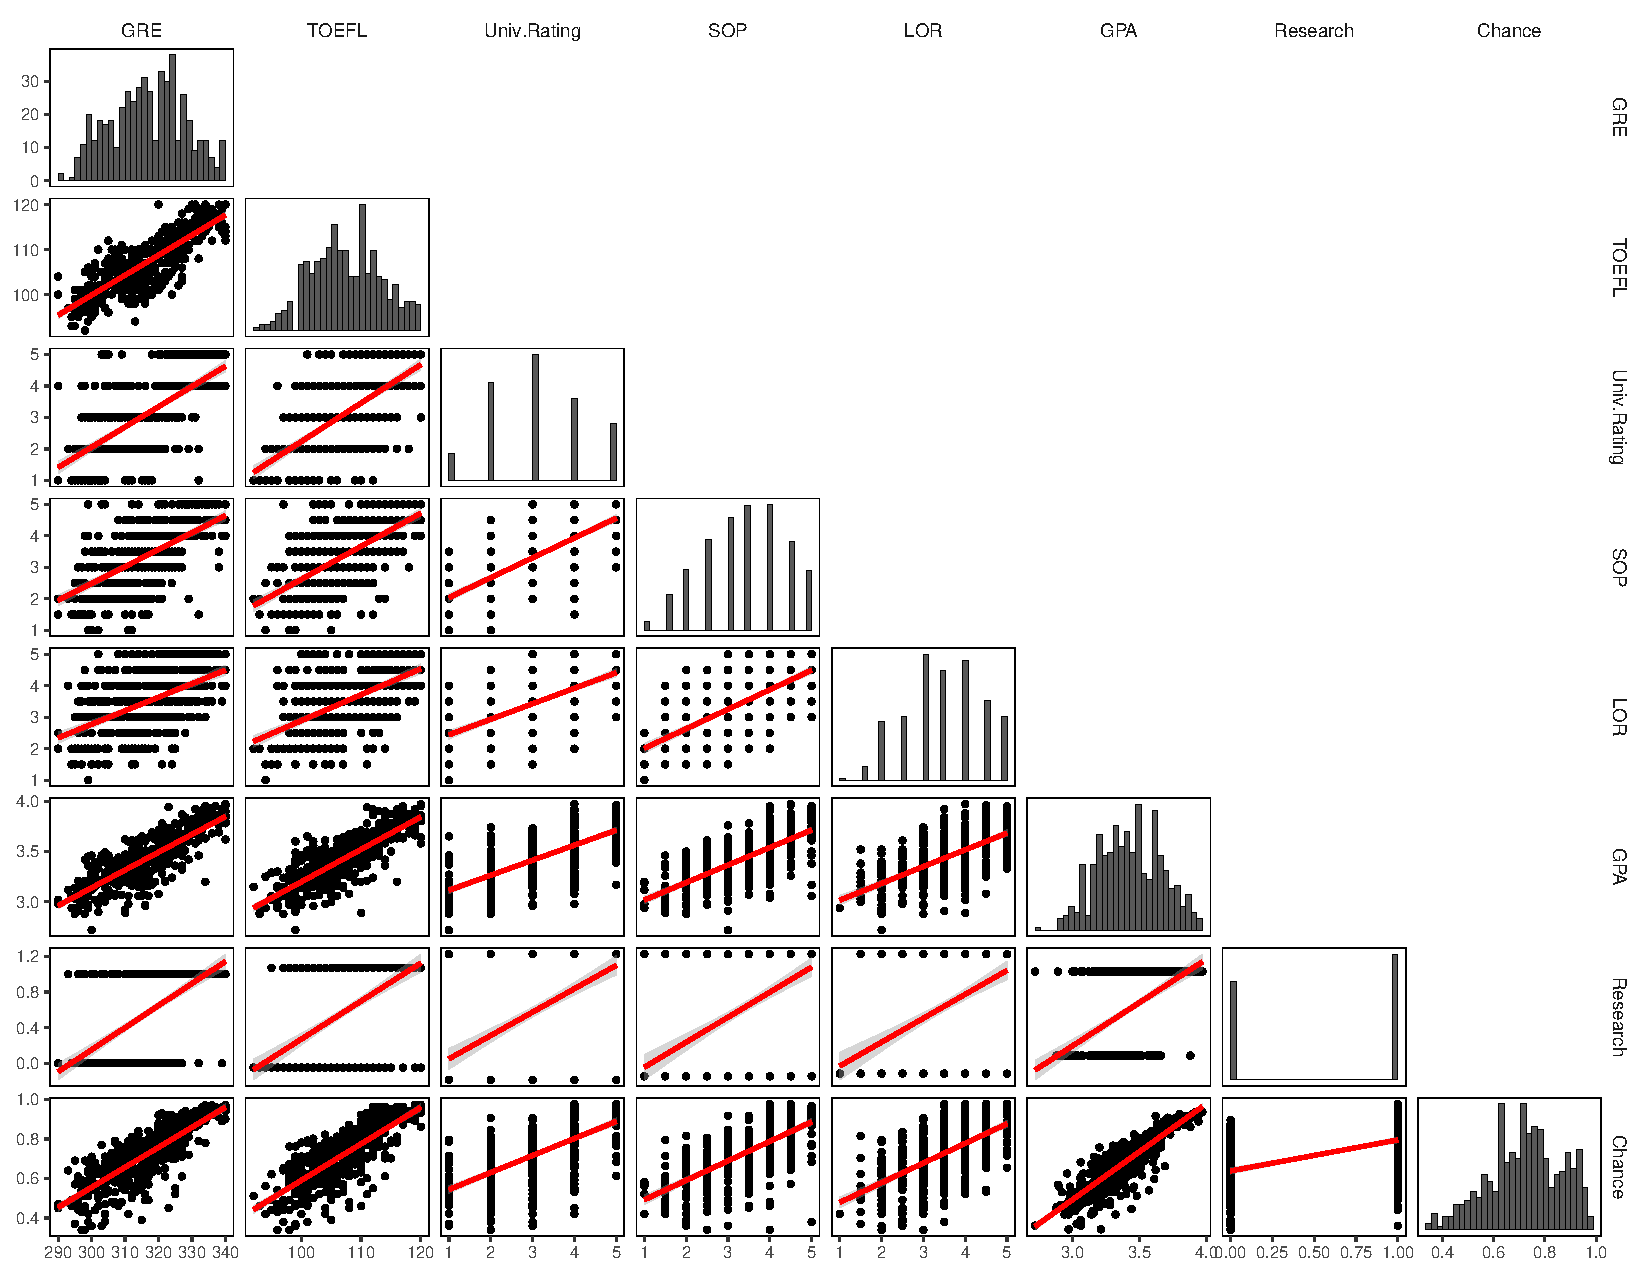
\includegraphics[width=4in, keepaspectratio]{./pic/matplot.pdf}\\
    \caption{矩阵散点图}
\end{figure}

矩阵散点图给出了数据分布的更多信息,可以看出数据并不符合正态分布。
利用随机森林\footnote{多棵决策树组成随机森林,根据特征在树上的位置估计其重要性,参见\ref{sec3.2}节}
对特征重要性排序,可见GPA确实是研究生申请中最重要的评价指标。

\begin{figure}[htb]
    \centering
    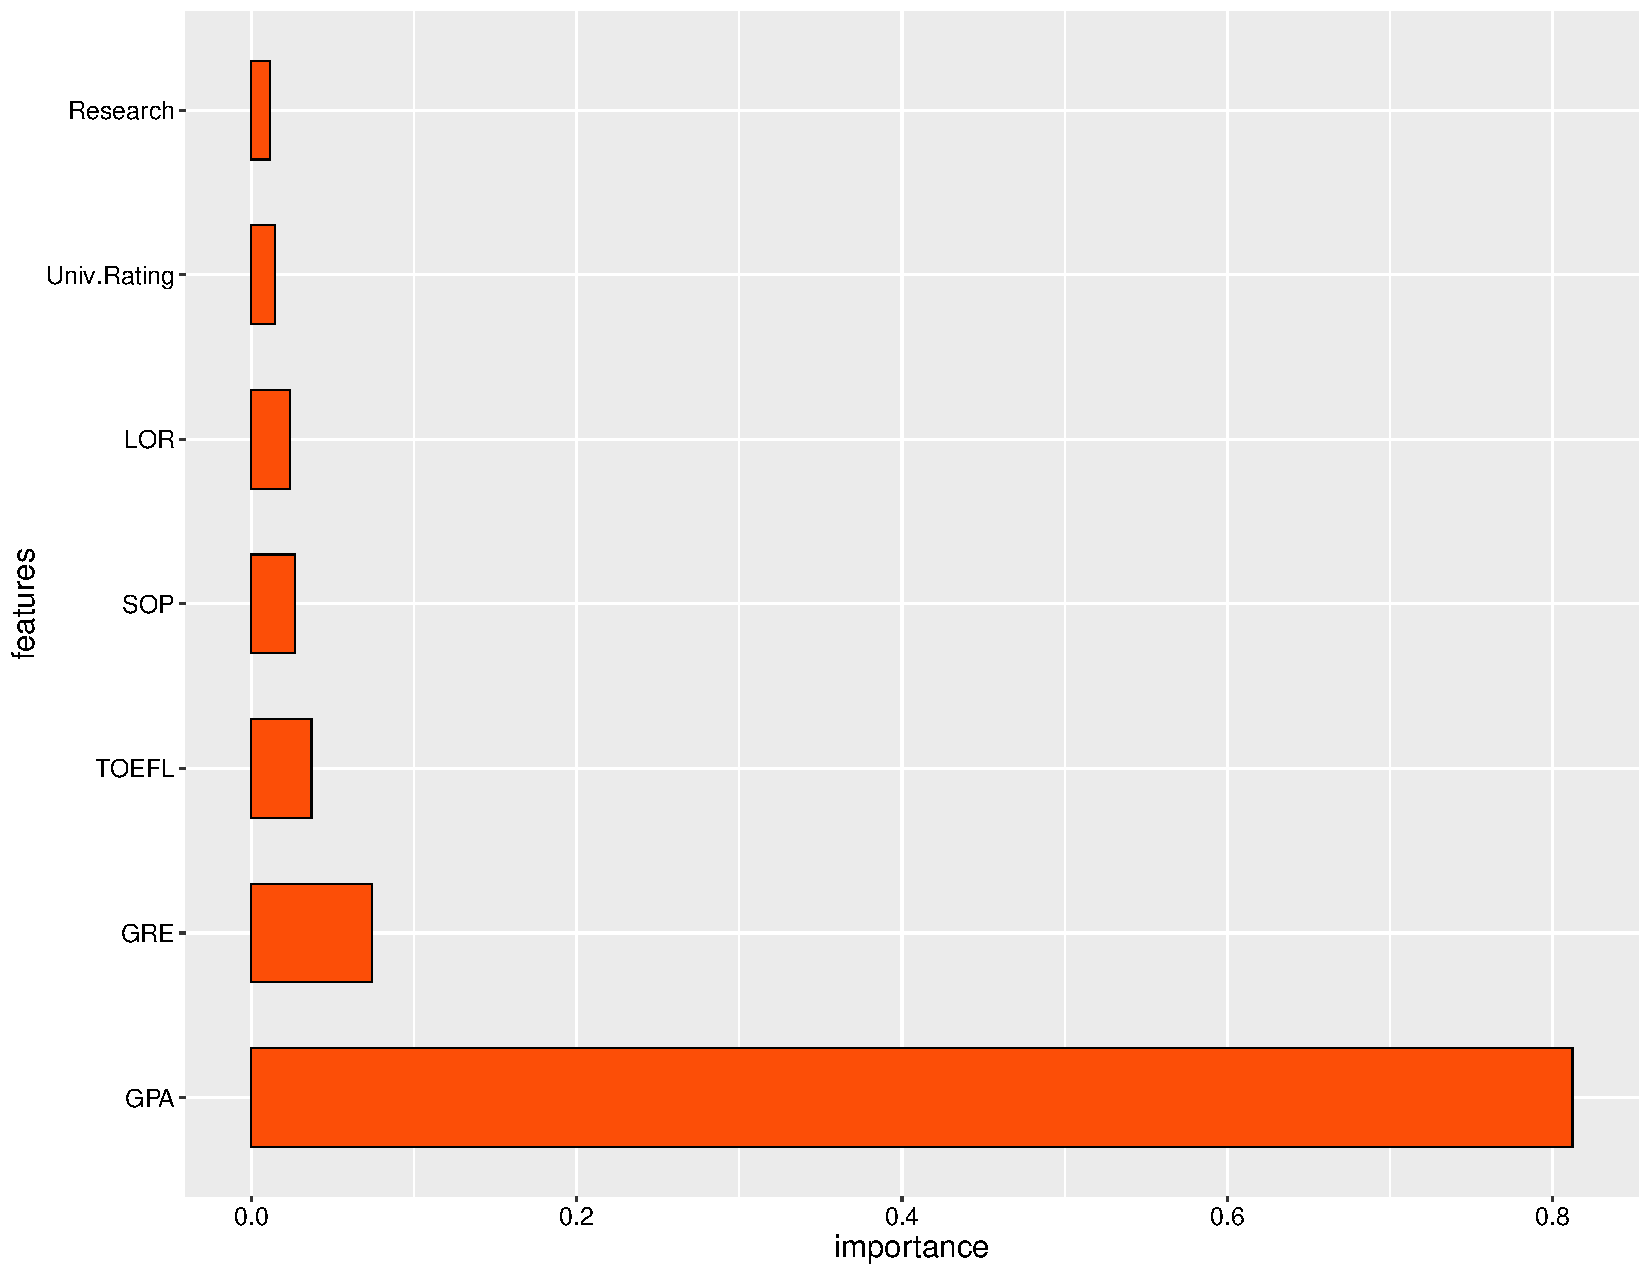
\includegraphics[width=4in, keepaspectratio]{./pic/rf.pdf}\\
    \caption{特征重要性条形图}
\end{figure}

\subsection{科研经历多重要?}

上一节的分析表明,科研经历是影响申请成功率的所有因素中最不重要的一个。
真的是这样吗?我们需要展开更深入的探索。

在全部500个样本中,有科研经历的有280个,没有科研经历的有220个。
是否参与科研与GPA之间存在明显的相关关系。

\begin{figure}[htb]
    \centering
    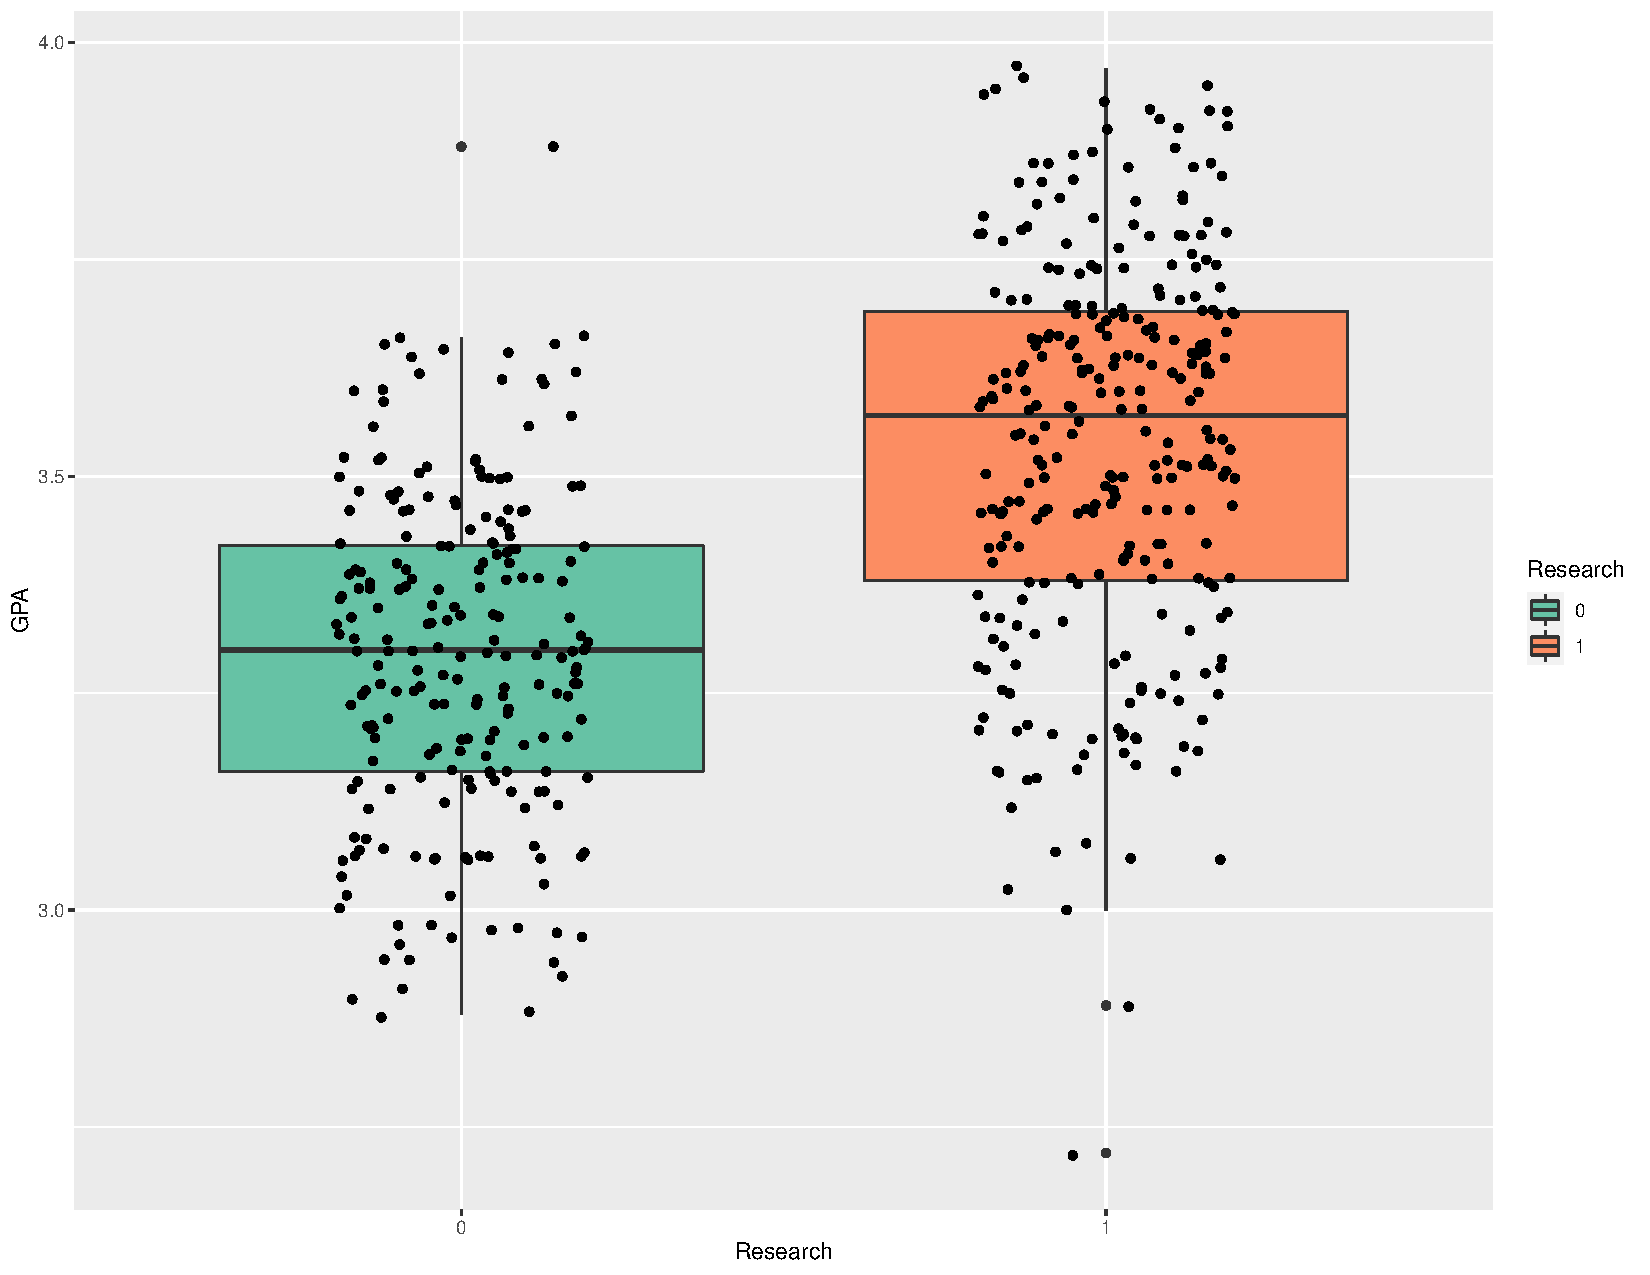
\includegraphics[width=3in, keepaspectratio]{./pic/GPAresearch.pdf}\\
    \caption{GPA vs. Research}
\end{figure}

对于来自不同评级大学的学生,科研经历带来的收益也不同。身处评级越高的本科院校,
参与科研带来的收益就越大。对于本科大学评级为4或5的申请者,
有科研经历和没有科研经历的平均录取概率相差10\%以上。
当然,这也是因为参与科研的
申请者往往学有余力。

\begin{figure}[htb]
    \centering
    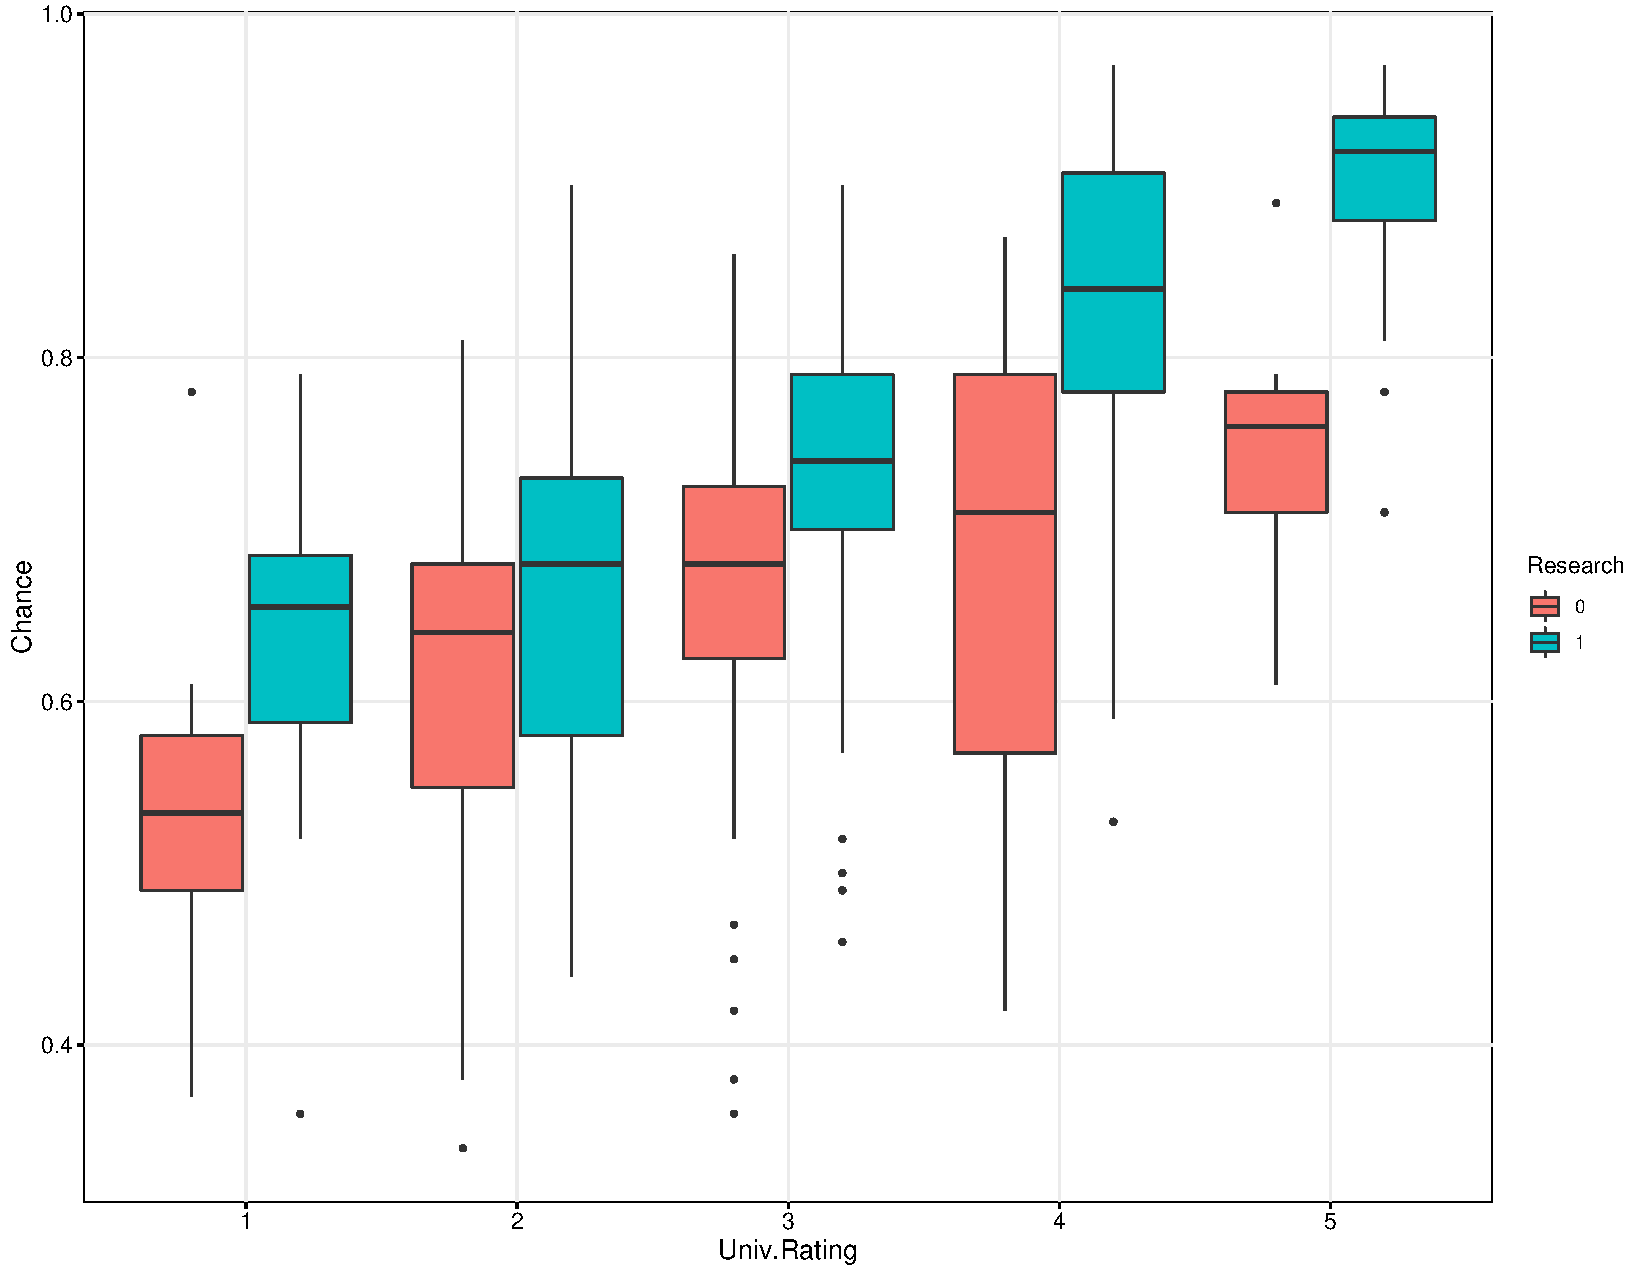
\includegraphics[width=4in, keepaspectratio]{./pic/univresearch.pdf}\\
    \caption{Univ.Rating vs. Research}
\end{figure}

\section{建模:研究生入学申请结果预测}

根据GPA,GRE等七项指标预测申请者被录取的概率,这是一个典型的回归问题。
为确保模型的可解释性,我选用了线性回归和决策树两种算法。

\subsection{线性模型}

用最小二乘法\footnote{实验表明OLS的拟合效果优于LASSO和岭回归.}
线性回归,
\begin{equation}\label{eq:1}
\begin{aligned}    
Chance &= 0.18\%\cdot GRE + 0.27\%\cdot TOEFL + 
        0.6\%\cdot Univ.Rating + 0.16\%\cdot SOP \\
       &\quad + 1.7\%\cdot LOR + 29.6\%\cdot GPA + 2.4\%\cdot Research - 128\%
\end{aligned}
\end{equation}根据公式,GPA每提高0.1,录取概率就提高2.96\%;
科研经历能使得录取概率提高2.4\%。可见,当提高GPA很困难时,积累一些科研经历也是不错的选择。

线性回归拟合的残差标准差约为5.9\%\footnote{指测试集上的RMSE,下同。}
,即通过这种方法计算出的录取概率与真实值间的平均偏差为5.9\%。

\subsection{决策树}\label{sec3.2}

决策树是基于树结构的一种机器学习模型,它在某种程度上模拟了人类的决策方式。
例如,我们要判断“这个西瓜是好瓜吗”,通常要进行一系列的子决策:我们先看“它的脐部是什么形态”,
如果是“稍凹”,则我们再看“它的根是什么形态?”,如果是“稍蜷”,我们再判断“它是什么颜色?”......
最后,我们得出结论,“这是个好瓜”。

\begin{figure}[htb]
    \centering
    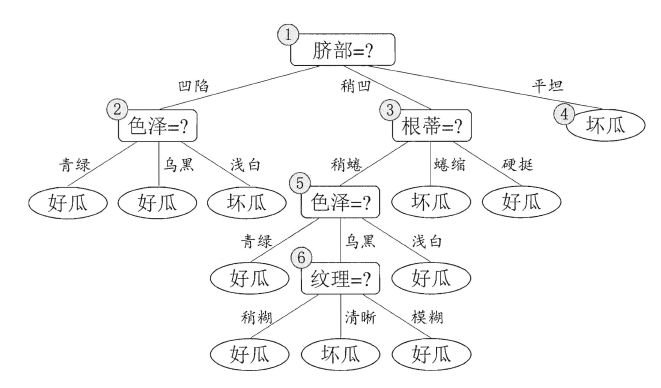
\includegraphics[width=4in, keepaspectratio]{./pic/decisionTreeDemo.png}\\
    \caption{选瓜问题的一棵决策树}
\end{figure}

注意到,决策过程中每一个子决策都是对事物某个特征的“测试”。
在决策树上越靠近树根的节点,其影响范围越大,它所对应的决策特征也就越重要。

如果决策树太浅,其信息量就会不足;如果太深,其可读性就会下降。设置深度为4,
构建研究生留学录取率的一颗决策树如图。

\begin{figure}[htb]\label{tree}
    \centering
    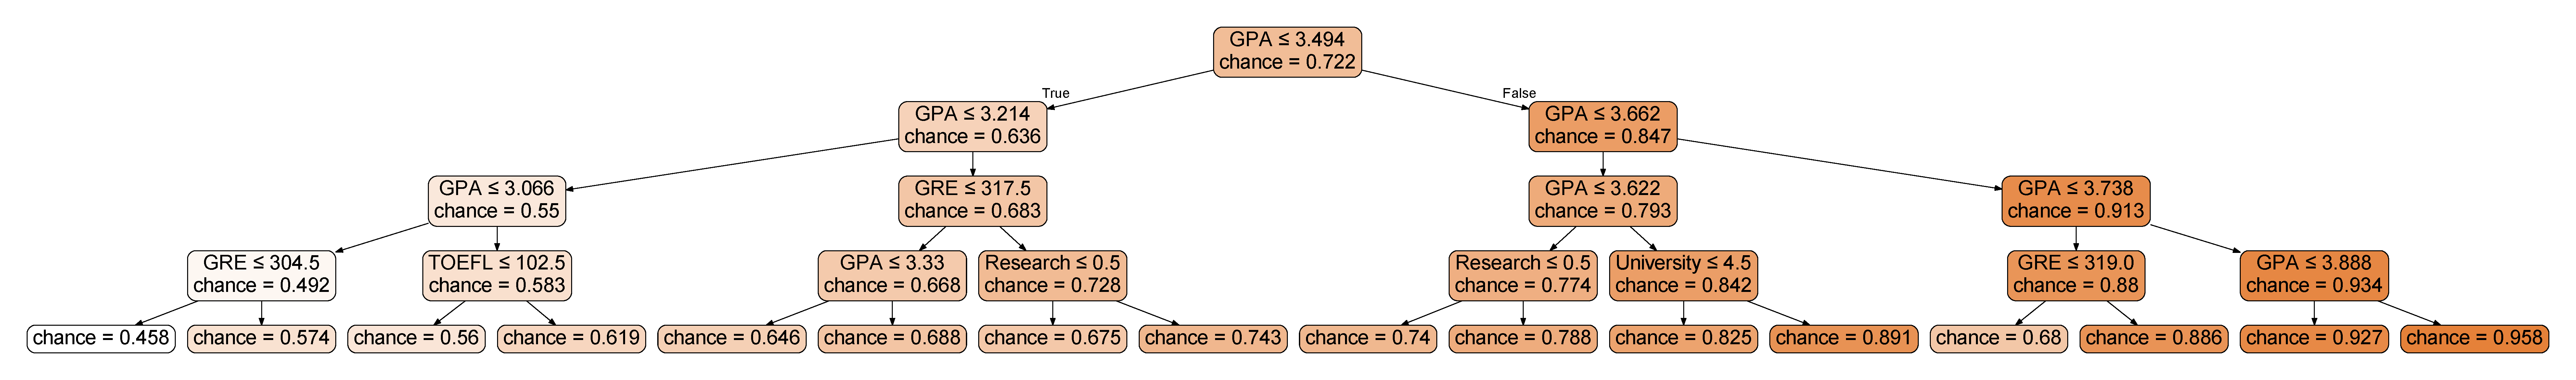
\includegraphics[width=6in, keepaspectratio]{./pic/tree.pdf}\\
    \caption{留学录取概率决策树}
\end{figure}

从根节点开始,如果满足节点上的决策条件就向左走,否则向右走,一直走到叶子节点上。
如果某申请者满足GPA=3.7,GRE=320,那他被录取的概率就是88.6\%。

通过图示决策树计算出的录取概率与真实值间的平均偏差为7.5\%。

\section{结论}

综上所述,研究生留学录取概率与申请者的GPA、GRE、TOEFL等七项指标均有密切关系,
其中GPA占决定性地位,其次是英语成绩(GRE、TOEFL)。

根据公式(\ref{eq:1}),可以认为有科研经历对录取概率的影响大致与GPA提高0.1或
TOEFL成绩提高10分相当。通过线性回归或决策树模型,可以在一定误差范围内预测录取概率,
其中线性回归的预测值更准确。

\section{改进方向与反思}

本项研究最大的困难,在于原始数据承载的信息量不足:
留学申请的成功率不只与我们掌握的七项指标有关,
科研经历不能简单地用有和没有来概括,所谓“录取概率”的现实意义不明。
这些问题严重影响了研究结果的实用性。

要改善这些问题,只能从数据收集的方法上着手:
我认为,应当在清华本科毕业年级中展开调查,把申请者专业背景,申请院校等因素纳入考虑
,以是否被录取作为观测指标,保证数据的客观性,这是后续研究所有现实意义的基础。

\end{document}